\chapter{Background}

% A more extensive coverage of what's required to understand your
% work. In general you should assume the reader has a good undergraduate
% degree in computer science, but is not necessarily an expert in
% the particular area you've been working on. Hence this chapter
% may need to summarize some ``text book'' material.

% This is not something you'd normally require in an academic paper,
% and it may not be appropriate for your particular circumstances.
% Indeed, in some cases it's possible to cover all of the ``background''
% material either in the introduction or at appropriate places in
% the rest of the dissertation.

This chapter reviews background relevant to the remainder of this dissertaion.
The scope includes an overview of music theory and automatic composition
and also includes coverage of sequence probability models.

\section{Music theory}

Music theory a branch of musicology concerned with the study of the rules and
practices of music. While the general field includes study of acoustic
qualities such as timbre and waveform synthesis, our work is concerned with
modelling the musical composition itself rather than acoustic features. This is
justified because acoustic features are more closely related to a particular
reproduction (e.g. the skill of the performers, quality of the instruments)
and are likely to vary significantly across different performances. Indeed,
references to a piece of music generally refer to the underlying composition
itself rather than any particular performance of the piece. This suggests
that the composition itself is more significant and hence a more desirable
modeling target.

We refer refer to a musical composition as a \textbf{score}, which we formally
define to be an ordered sequence of \textbf{note}s. Each note possesses a pitch
(i.e.\ frequency) and a time interval (i.e.\ start and stop times) and
represents an instruction for the performer to articulate the given pitch at
the start time and hold the note until the stop time. Multiple notes may
overlap in time, in which case all notes are to be played simultaneously.

\subsection{Pitches and tuning systems}

The \textbf{pitch} of a note refers to the frequency of sound used in its
reproduction and the difference between two pitches is called a \textbf{pitch
interval}. A fundamental pitch interval in Western music is the
\textbf{octave}, which is defined to be the interval between a frequency and
its double.

While in theory an uncoutable number of pitches are available because
frequencies are real-valued and hence there are uncountably many, tuning
systems are oftentimes employed to restrict the set of available pitches in
order to simplify composition, analysis, and reproduction. A \textbf{tuning
system} restricts the available pitch intervals, limiting the possible pitches
to a discrete set.

Western music commonly uses a tuning system called \textbf{12-TET} (12 tone
equal temperament) tuning, which divides an octave into 12 \textbf{pitch
classes} ($C$, $C\#/D\flat$, $D$, $D\#/E\flat$, $E$, $F$, $F\#/G\flat$, $G$,
$G\#/A\flat$, $A$, $A\#/B\flat$, $B$) all equally spaced on a logarithmic
scale. Each pitch class represents an equivalence class of frequencies which
all differ by an integral number of octaves (i.e. are doublings/halvings of
each other). This means that unambiguously specifying a pitch requires
specifying both a pitch class and an octave. Common practice numbers octaves
with respect to a standard sized keyboard, where the key corresponding to the
\textbf{middle $C$} note is referred to as $C_5$ because it is $5$ octaves
above the lowest $C$ key. The interval between two adjacent pitch classesis
called a \textbf{half step} or \textbf{half tone} and two half steps are called
a \textbf{whole step/tone}.

In our work, we restrict attention to 12-TET tuning because it is the most
common tuning system employed by Western composers over the last 

Note that while 12-TET restricts the available pitches to a discrete set, it
lacks specification of a reference pitch frequency and hence does not yield a
correspondance between pitches and frequencies. This degree of freedom gives
rise to \textbf{transposition invariance}: a score of music can be offset by a
constant frequency without altering characteristics arising from the pitches
present in the music. In modern practice, the general tuning standard of $A440$
defines a reference frequency of 440 Hz for the $A$ pitch class directly above
middle C.

\subsection{Tonal music}

Tonal music is characterized by the prevalence of one pitch class (the
\textbf{tonic}) around which the melody and harmony are built. 

A basic concept
within tonal music is the \textbf{scale} which defines a subset of pitch
classes that are ``in key'' with respect to the tonic. Two fundamental scales
are the major (with step pattern whole-whole-half-whole-whole-whole-half) and
minor scales (whole-half-whole-whole-half-whole-whole). The choice of tonic and
scale is referred to as the \textbf{key}and a change in key during a piece is
called a \textbf{modulation}Many musical phenomena such as stability,
expectation, and resolution can be attributed to tonal characteristics.

The \textbf{tempo} of a piece refers to its speed or pace and is measured by
beats per minute. In 4/4 time signature, a \textbf{quarter note} or
\textbf{crotchet} denotes the time interval between two beats. In addition to
pitch quantization, durations are also commonly quantized to subdivisions and
multiples of a crotchet.

\subsection{Notation}

We consider note duration, time, and velocity. We neglect changes in timing
(e.g. ritardandos), dynamics (e.g. crescendos), and stylistic notations (e.g.
accents, staccatos, legatos).

\emph{Piano roll} music transcriptions are quantized both in time ($t \in T$)
and note frequencies ($n \in N$). frequencies quantized to a piano roll.
\todo{Motivate quantization with Western music}.

We can represent a piano roll transcription as a high-dimensional vecctor
$X_{t,n} \in \RR^{|T| \times |N|}$ where $X_{t,n}$ denotes the note
velocities for note $n$ at time $t$.

\section{Automatic composition}

Algorithmic composition is the application of a well-defined algorithmic
procedure to compose music.

An interesting question regarding creativity: if an algorithm faithfully reproduces
an artist's creative process, what is the difference between music produced by the artist
and music produced by the algorithm?

\section{Sequence probability modelling}

Generating a "Bach-like" piece of music can be understood as drawing a random
sample from a distribution over musical scores which is statistically similar
to Bach's own compositions. Thus, we interpret the problem as one of
\emph{categorical sequence modeling}.

This type of problem has been well studied. In speech recognition, language
models parameterizing distributions over sentences are used as priors to refine
transcriptions.

However, since our model has to be able to generate Bach, we must be able to
sample from it. This rules out a broad class of sequence models, including
back-off N-grams and other interpolated language models.

Fortunately, low order N-grams and standard HMM-based models are sampleable and
thus can be used as baselines.

\subsection{Feedforward neural networks}

Feedforward neural networks are a parametric model capable of approximating a
broad range of functions \todo{Include universal approximation}. Their capacity
to model a diverse range of functions make them an appealing model for complex
unknown probability distributions.

A feedforward neural network is the composition of a sequence of layers, each
taking some \textbf{inputs} $\vec{x}$ and performs an affine transformation $\vec{z} =
\matr{W} [\vec{x}, 1]^\tp$ to yield \textbf{activations}. The activations are then
passed through an \textbf{activation function}, which applies an elementwise
nonlinearity $\sigma : \RR \to [L,U]$ squashing the outputs to into some connected bounded
subset $[L,U] \subset \RR$. A common choice is the logistic function $\sigma(z)
= \frac{1}{1+\exp{-z}}$, which squashes $\vec{y} \in [0, 1]$. Other choices
include $\sigma = \tanh$, in which case $[L, U] = [-1, 1]$.

It is common to represent feedforward neural networks as directed acyclic
graphs (\autoref{fig:nn-layer}). Here, each node denotes a data value and
an edge from $s$ to $t$ notates that the value at $s$ is used to compute the
value at $t$.

\begin{figure}[htpb]
    \centering
    \def\layersep{2.5cm}

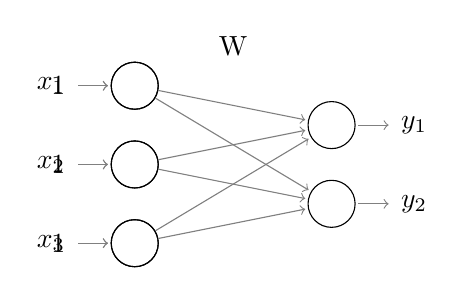
\begin{tikzpicture}[shorten >=1pt,->,draw=black!50, node distance=\layersep]
    \tikzstyle{every pin edge}=[<-,shorten <=1pt]
    \tikzstyle{neuron}=[circle,draw=black!100, minimum size=17pt,inner sep=0pt]
    \tikzstyle{input neuron}=[neuron];
    \tikzstyle{output neuron}=[neuron];
    \tikzstyle{hidden neuron}=[neuron];
    \tikzstyle{annot} = [text width=4em, text centered]

    % Draw the input layer nodes
    \foreach \name / \y in {1,...,3}
        \ifthenelse{3 = \y}{
            \node[input neuron, pin=left:$1$] (I-\name) at (0,-\y) {};
        }{
            \node[input neuron, pin=left:$x_\y$] (I-\name) at (0,-\y) {};
        }; % (*)

    % Draw the output layer node
    \foreach \name / \y in {1,...,2}
        \path[yshift=-0.5cm]
            node[output neuron,pin={[pin edge={->}]right:$y_\y$}] (O-\name) at (\layersep,-\y cm) {};

    % Connect every node in the input layer with every node in the
    % output layer
    \foreach \source in {1,...,3}
        \foreach \dest in {1,...,2}
            \path (I-\source) edge (O-\dest);

    \node[annot,above of=I-1, xshift=0.5*\layersep, node distance=0.5cm] {W};
\end{tikzpicture}

    \caption{Single feedfoward neural network layer}
    \label{fig:nn-layer}
\end{figure}

Multiple layers can be composed together by treating the outputs from the previous layer
as the inputs to the next layer. \autoref{fig:ffw-nn} illustrates this on a 2-layer
feedforward neural network where the outputs of the first layer are used as the
inputs to the second layer (i.e. $x^{(1)} = y^{(0)}$).

\begin{figure}[htbp]
    \centering
    \def\layersep{2.5cm}

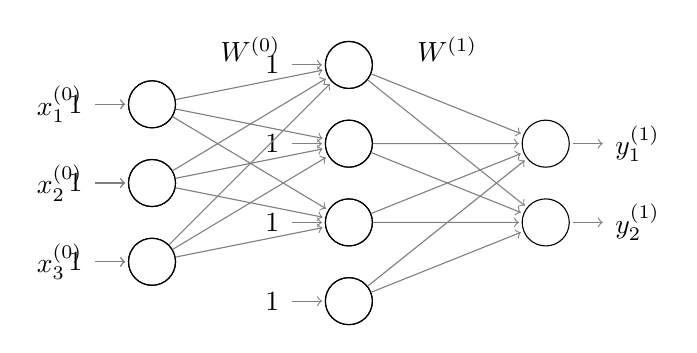
\begin{tikzpicture}[shorten >=1pt,->,draw=black!50, node distance=\layersep]
    \tikzstyle{every pin edge}=[<-,shorten <=1pt]
    \tikzstyle{neuron}=[circle,draw=black!100, minimum size=17pt,inner sep=0pt]
    \tikzstyle{input neuron}=[neuron];
    \tikzstyle{output neuron}=[neuron];
    \tikzstyle{hidden neuron}=[neuron];
    \tikzstyle{annot} = [text width=4em, text centered]

    % Draw the input layer nodes
    \foreach \name / \y in {1,...,3}
        \ifthenelse{3 = \y}{
            \node[input neuron, pin=left:$1$] (I-\name) at (0,-\y) {};
        }{
            \node[input neuron, pin=left:$x^{(0)}_\y$] (I-\name) at (0,-\y) {};
        };

    % Draw the hidden layer nodes
    \foreach \name / \y in {1,...,4}
        \ifthenelse{4 = \y}{
            \path[yshift=0.5cm]
                node[hidden neuron, pin=left:$1$] (H-\name) at (\layersep,-\y cm) {};
        }{
            \path[yshift=0.5cm]
                node[hidden neuron] (H-\name) at (\layersep,-\y cm) {};
        };

    % Draw the output layer node
    \foreach \name / \y in {1,...,2}
        \path[yshift=-0.5cm]
            node[output neuron,pin={[pin edge={->}]right:$y^{(1)}_\y$}] (O-\name) at (2*\layersep,-\y cm) {};

    % Connect every node in the input layer with every node in the
    % hidden layer.
    \foreach \source in {1,...,3}
        \foreach \dest in {1,...,3}
            \path (I-\source) edge (H-\dest);

    % Connect every node in the hidden layer with the output layer
    \foreach \source in {1,...,4}
        \foreach \dest in {1,...,2}
            \path (H-\source) edge (O-\dest);

    % Annotate the layers
    \node[annot,above of=I-1, xshift=0.5*\layersep, node distance=0.7cm] (hl) {$W^{(0)}$};
    \node[annot,right of=hl] {$W^{(1)}$};
\end{tikzpicture}

    \caption{2-layer feedforward neural network}
    \label{fig:ffw-nn}
\end{figure}

\todo{Plug to deep learning}

\subsubsection{Modeling probability distributions}

A neural network can be used to model the distribution of a categorical random
variable $o$ by treating the final layer activations $\vec{z}^{(L)}$ as the
energies of a Boltzmann distribution (i.e.\ $\softmax$). This implies a
probability mass function on $o$ given by \autoref{eq:softmax}.

\begin{equation}
    \label{eq:softmax}
    P(o = k | \vec{z}^{(L)}) = \frac{\exp{-z^{(L)}_k}}{ \sum_{j} \exp{-z^{(L)}_j} }
\end{equation}

\subsubsection{Training with back-propogation}

Training neural networks is achieved using gradient descent methods, which
optimize parameters $\theta = \{W^{(i)} : 1 \leq i \leq L \}$ to minimize some
loss function $L(\vec{z}^{(L)}_{1:N}, \hat{o}_{1:N})$ between the network
outputs $\vec{z}^{(L)}_{1:N}$ and the true labels $\hat{o}_{1:N}$. For
probabilistic classification, a common choice is to assume independence
across training examples and use \textbf{cross-entropy loss}
(\autoref{eq:cross-entropy-loss}):

\begin{align}
    L(\vec{z}^{(L)}_{1:N}, \hat{o}_{1:N})
    &= \sum_{i=1}^{N} L(\vec{z}^{(L)}_i, \hat{o}_i) &\mbox{Independence across samples} \nonumber\\
    &= \sum_i \sum_k \delta_{\hat{o}_i,k} \log \frac{1}{P(o=k | \vec{y}_i^{(L)})} & \label{eq:cross-entropy-loss}
\end{align}

Gradient descent proceeds by using the Jacobian (i.e.\ gradient) $\nabla_\theta
L(\vec{z}^{(L)}_{1:N}, \hat{o}_{1:N})$ to iteratively update the network
parameters using successive first-order approximations (\autoref{eq:nn-training-iteration-scheme}).

\begin{align}
    \label{eq:nn-training-iteration-scheme}
    \theta^{(t+1)} = \theta^{(t)}
    - \eta_t \left[ \nabla_\theta L(\vec{z}^{(L)}_{1:N}, \hat{o}_{1:N}) \right]_{\theta = \theta^{(t)}}
\end{align}

Variants of \autoref{eq:nn-training-iteration-scheme} which adaptively set the
step size $\eta_t$ or incorporate/estimate the Hessian $\nabla^2_{\theta}
L(\cdot, \cdot)$ can yield performance when applied to neural network training.
However, their discussion is out of scope. \todo{Discuss RMSprop?}

To apply \autoref{eq:nn-training-iteration-scheme}, the gradient $\nabla_\theta
L(\vec{z}^{(L)}_{1:N}, \hat{o}_{1:N})$ must be computed. This can be
accomplished using \textbf{backpropogation} \todo{cite}, an algorithm which
exploits the independence structure to avoid unnecessary computations and make
gradient computations tractable.

Let $\delta^{(l)}_{j} = \frac{\pd L(\vec{z}^{(L)}_{1:N}, \hat{o}_{1:N})}{\pd
z^{(l)}_j}$ be the partial derivative of the loss with respect to the $j$th
activation of layer $l$. For the final $L$th layer, cross-entropy loss
with a Boltzmann distribution yields

\begin{align*}
    \delta^{(L)}_{j}
    &= - \sum_{i=1}^{N} \sum_{k} \frac{\pd}{\pd z^{(L)}_j} \delta_{\hat{o}_i,k} \log P(o=k | \vec{z}^{(L)}_i ) &\mbox{\autoref{eq:cross-entropy-loss}} \\
    &= \sum_{i=1}^{N} \left( P(o=k | \vec{z}^{(L)}_i ) - y_i \right) & \mbox{Softmax derivative}
\end{align*}

For earlier layers $l < L$, we have
\begin{align}
    \delta^{(l)}_{j}
    &= \sum_k \frac{\pd L(\vec{z}^{(L)}_{1:N}, \hat{o}_{1:N})}{\pd z^{(l+1)}_k}
    \frac{\pd z^{(l+1)}_k}{\pd z^{(l)}_j}\\
    &= \sum_k \delta^{(l+1)}_k
    \frac{\pd}{\pd z^{(l)}_j} \left( \matr{W}^{(l+1)} [\sigma(z^{(l)}), 1]^\tp \right)_k \\
    &= \sum_k \delta^{(l+1)}_k
    \matr{W}^{(l+1)}_{k,j} \sigma'(z^{(l)}_j) \label{eq:backprop}
\end{align}
This expression can be vectorized using the Hadamard product (elementwise multiplication), which
improves performance due to CPU cache locality and coalesced memory loads: \todo{DO THIS}
\begin{align}
    \circ
\end{align}
This recursion can be iterated until $l \to 0$.

The back-propogation algorithm consists of two steps:
\begin{enumerate}
    \item \emph{Forward pass}: Using current model parameters $\theta^{(t)}$,
        feed the data into the network to compute the activations $\vec{z}^{(l)}$,
        $1 \leq l \leq L$
    \item \emph{Backward pass}: Recursively iterate \autoref{eq:backprop}
        to compute $\vec{\delta}^{(l)}$, $1 \leq l \leq L$ using the activations
        $\vec{z}^{(l)}$ obtained from the forward pass
\end{enumerate}

After the backwards pass, gradients with respect to model parameters are easily obtained
\begin{align}
    \frac{\pd L}{\pd W^{(l)}_{i,j} }
    &= \sum_k \frac{\pd L}{\pd z^{(l+1)}_k} \frac{\pd z^{(l+1)}_k}{\pd W^{(l)}_{i,j}} \\
    &= \sum_k \delta^{(l+1)}_k z^{(l)}_j
\end{align}

Some appealing properties of backpropogation:
\begin{itemize}
    \item Efficient exploitation of the computation graph: chain rule expansions
        are constrained by the computation graph, improving efficiency
        because factors which don't contribute to a given $\delta^{(l)}$
        are neglected in the recursion
    \item Implementation using local rules: the forward/backward pass
        at any layer $l$ only requires knowledge of $z^{(l)}$, $\delta^{(l+1)}$,
        and the derivative of the activation $\sigma'$. As all these quantities are localized
        to one layer, this permits modular implementations where a node which can be back-propped
        through needs only implement a \texttt{forward()} method which computes activations
        given inputs and a \texttt{backward()} method which computes $\delta^{(l)}$ given
        activations.
\end{itemize}

\todo{Talk about how localization gives rise to computation graph and autodiff}

\subsection{Recursive neural networks}

Recursive neural networks (RNNs) are a generalization of feedforward neural
networks which introduce recurrent connections. This implies that its graphical
representation is no longer acyclic.

\todo{Figure for RNN with loops}

Given an input $\vec{x}_{1:T}$, a RNN can be unrolled into an equivalent feed-forward
network with tied weights:
\begin{figure}[htpb]
    \centering
    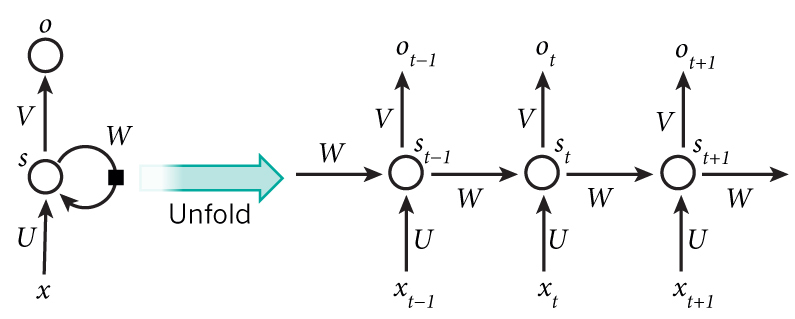
\includegraphics[width=0.8\linewidth]{Figures/rnn.jpg}
    \caption{\todo{Redraw in xy}}
\end{figure}
We can view the recurrent data $s_t$ as \textbf{state} which evolves
over consecutive \textbf{frames} $x_t$ according to dynamcis defined
by the RNN.

Mathematically, a RNN is defined by the equations
\begin{align}
    \s_t &= f(\U \x_t + \W \s_{t-1}) \\
    \o_t &= \softmax( \V \s_t)
\end{align}

$f$ is usually $\tanh$ or ReLU.

The advantages of RNNs over feedforward networks include:
\begin{itemize}
    \item Ability to handle variable-length inputs: the RNN can be unrolled an arbitrary
        number of times to accomodate inputs $\vec{x}$ of different length
    \item Fixed dimension embeddings: after processing the entirety of an input
        sequence, the state of the RNN can be used as a fixed dimension embedding
        representing the input
                \begin{figure}[htpb]
                    \centering
                    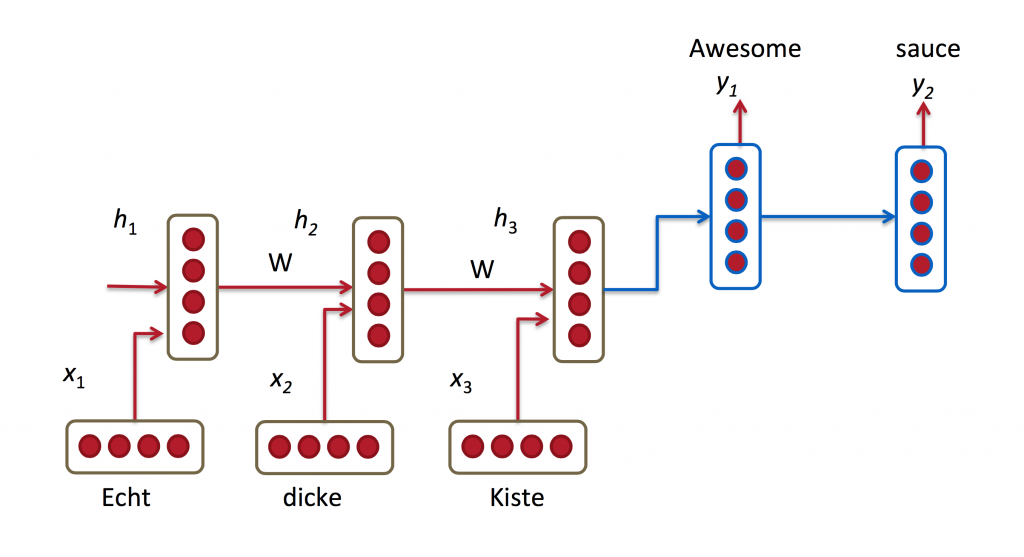
\includegraphics[width=0.8\linewidth]{Figures/rnn-mt.png}
                    \caption{\todo{Redraw in xy}}
                \end{figure}
    \item Sequential processing: the order of $\vec{x}_{1:T}$ will affect the state
        trajectory $s_{1:T}$, enabling the model to capture time-dependent dynamics
        within the input sequences
    \item Memory over time: the state $s \in \RR^D$ can take on an uncountably infinite
        number of values, allowing it to potentially act as memory which summarizes
        \emph{all} of the input up to the current time
\end{itemize}

\subsubsection{Comparison against HMMs}

Hidden Markov Models (HMMs) are another popular probabilistic model for
sequental data. \todo{Define HMMs}

While RNNs are similar HMMs in that both model the conditional distribution of
next frames given the previous context. However, RNNs additionally pass along
"hidden state" which summarizes contextual information from a potentially
infinite context window.

\subsubsection{Vanishing gradients and LSTMs}

In practice, it is observed that the hidden state does not capture long range
dependencies well and tend to suffer from vanishing/exploding gradient during
training. LSTMs are an improved RNN architecture which solve both of these
problems by introducing gates on the inputs, hidden state, and outputs. GRUs are
a variation of LSTMs which ties the weights to the input and forget gates.

\todo{Nando's slides for exploding gradient and how LSTM gates fix it}

